\chapter{Gas Electron Multiplier Detectors}
\label{chap:II-1-gem}

  In 1968, G. Charpak revolutionized the field of tracking detectors by introducing the Multiwire Proportional Chamber (MWPC). MWPCs were more reliable than the existing single-wire gas counters providing a higher sub-mm resolution and rate capabilities up to fluxes of several MHz mm$^{-2}$. Developments of manufacturing techniques and high-density electronics led to a new generation of detectors fulfilling the needs of high-energy physics experimentation. However, their use in high-luminosity experiments revealed some intrinsic weaknesses: the mechanical design of the chamber limits the spacial resolution; long ion drift times affect the efficiency of the detector at high fluxes; solid deposits agglomerate on the wires due to aging, and induce sparks in the chamber. \\

  Twenty years later, Micro-Strip Gas Counters (MSGCs) \cite{Alunni:254631} were developed using photolithographic processes to engrave anode and cathode strips on an insulating support. Both the position resolution and the rate capability were increased by several orders of magnitude. Unfortunately, the detectors were prone to the effect of aging and discharges, irremediably damaging the counters. \\

  The success of the MSGCs led to the development of Micro-Pattern Gas Detectors (MPGDs) less susceptible to discharges and offering comparable performances. They use micro pattern structures to amplify the signal and reduce the probability of sparks. Two technologies have proven to be operational: the MICRO-MEsh GASeous structure (MICROMEGAS) \cite{Giomataris:299159} and the Gas Electron Multiplier (GEM) \cite{SAULI1997531}. \\

  Already in use in the COMPASS and TOTEM experiments at CERN, GEM detectors have proven to meet the requirements of high-luminosity environments. In 2009, a dedicated R\&D program was launched to study the feasibility of the installation of GEMs in the muon spectrometer of CMS to instrument the positions left vacant by RPCs. Six years later, the so called GE1/1 muon detector upgrade project was approved by CMS to be installed during LS2.

  \section{Motivations for the GE1/1 Upgrade}

    During LS2, that will take place in 2019-2020, the CMS GEM collaboration \cite{Colaleo:2021453} will install an additional set of muon detectors in CMS in the 1.6 < |$\eta$| < 2.2 region. The so-called GE1/1 detectors will be installed near the ME1/1 CSC station as shown in Figure \ref{fig:II-1-ge11} which highlights the location of the chambers within the muon spectrometer in a longitudinal view of a quadrant of CMS. \\

    \begin{figure}[t!]
      \centering
      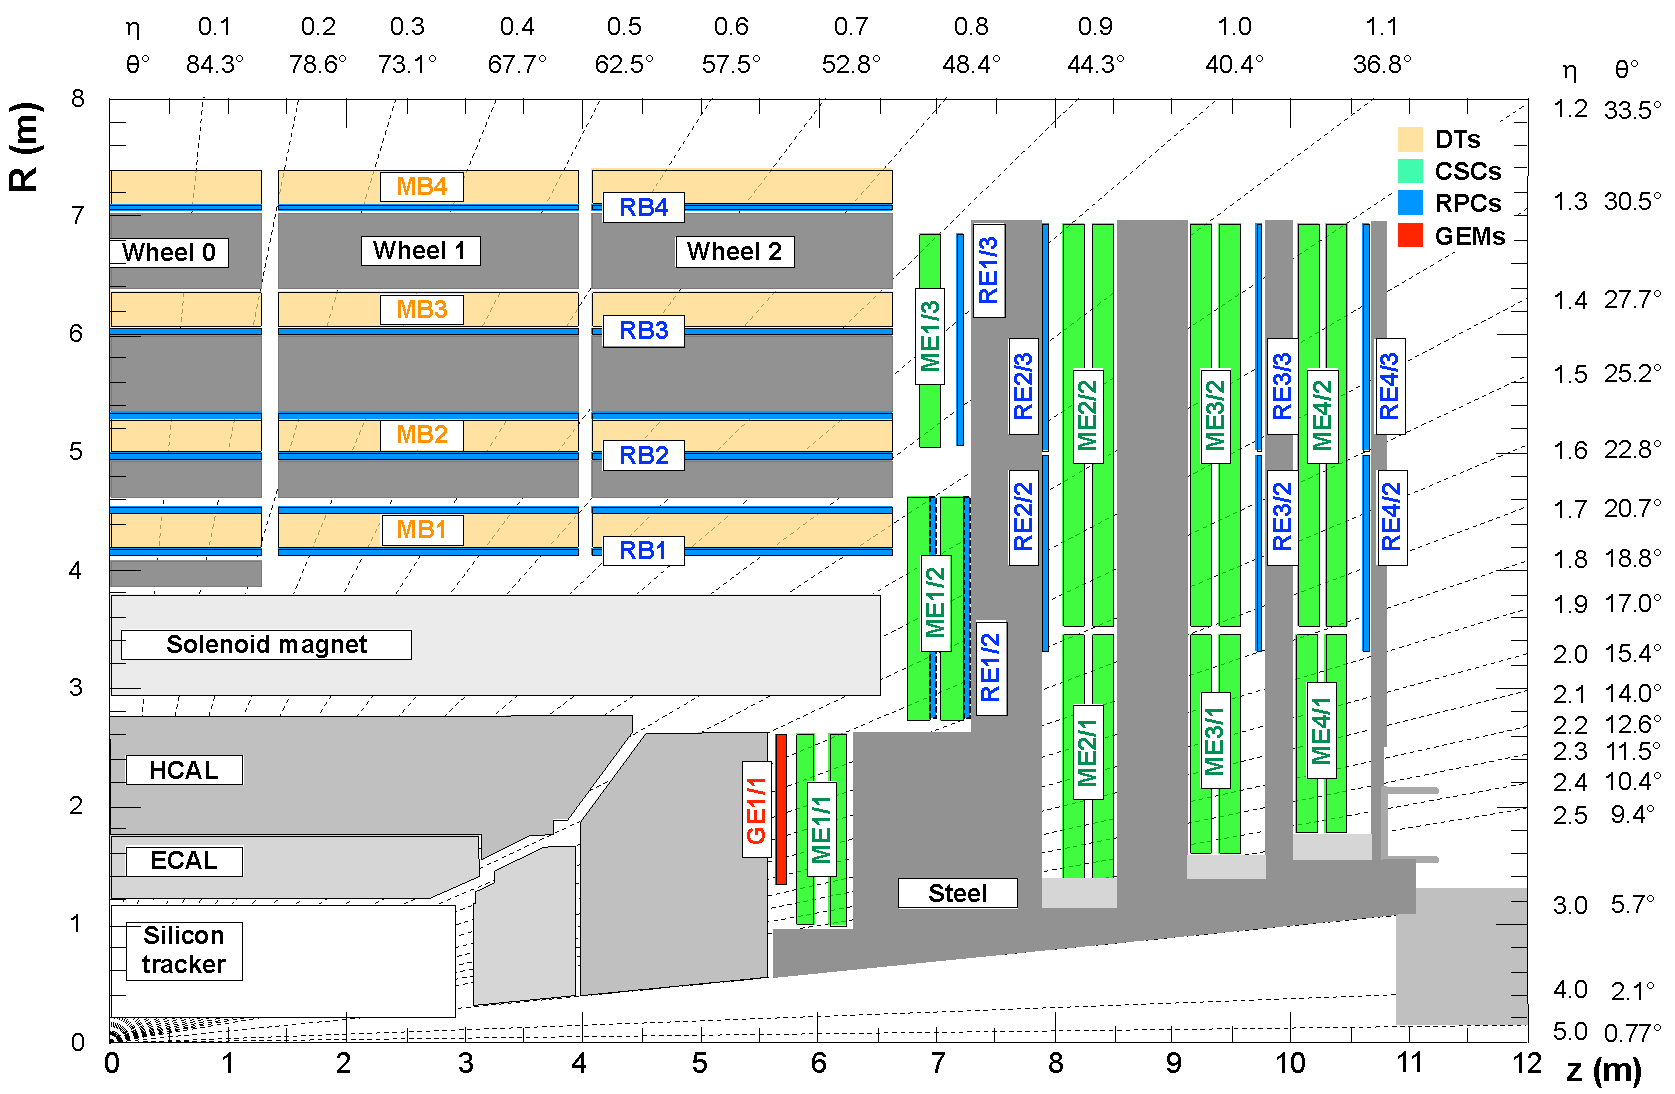
\includegraphics[width=\textwidth]{img/II-1-gem/ge11-quadrant.pdf}
      \caption{Longitudinal view of a quadrant of CMS highlighting the location of the GE1/1 detectors colored in red within the muon spectrometer. DTs are represented in yellow, CSCs in green, and RPCs in blue \cite{Colaleo:2021453}.}
      \label{fig:II-1-ge11}
    \end{figure}

    The main motivation for the installation of GE1/1 is the significant impact it has on the triggering system of CMS. Left as is, the performance of the current system would degrade in the coming years with the increase in instantaneous luminosity due to the rate limitations of the ME1/1 station exposed to an intense flux of particles. Muon triggering will in turn suffer from a degradation in the resolution on the transverse momentum, p$_T$. As muon triggers are limited in bandwidth to a fraction of the total allocated bandwidth of the trigger, typically 5 kHz for the single muon trigger, they must set a cut on the minimum p$_T$ of the muons (around 20 GeV). In the scenario where the muon spectrometer remains unmodified, the threshold would have to be raised to p$_T$ $ \approx $ 30 GeV which would be a considerable drawback in terms of physics analysis, decreasing the acceptance by more than 35\% for given channels. \\

    In order to prevent the degradation of the trigger system, the GEM collaboration investigated the possibility to use the bending angle of tracks between GE1/1 and ME1/1 to estimate the p$_T$ of muons, which trajectory is curved by the magnetic field. Figure \ref{fig:II-1-csc-bending} shows on the left the lever arm given by the 20 cm to 46 cm distance between the two detectors. The variation in distance corresponds to "close" and "far" chambers which are staggered in order to allow for some overlap and avoid dead space. From this, the picture on the right displays the discrimination power between 5 GeV/c and 20 GeV/c muons. \\

    \begin{figure}[t!]
      \centering
      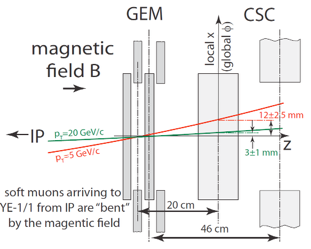
\includegraphics[width=0.45\textwidth]{img/II-1-gem/gem-csc-bending-1.png}
      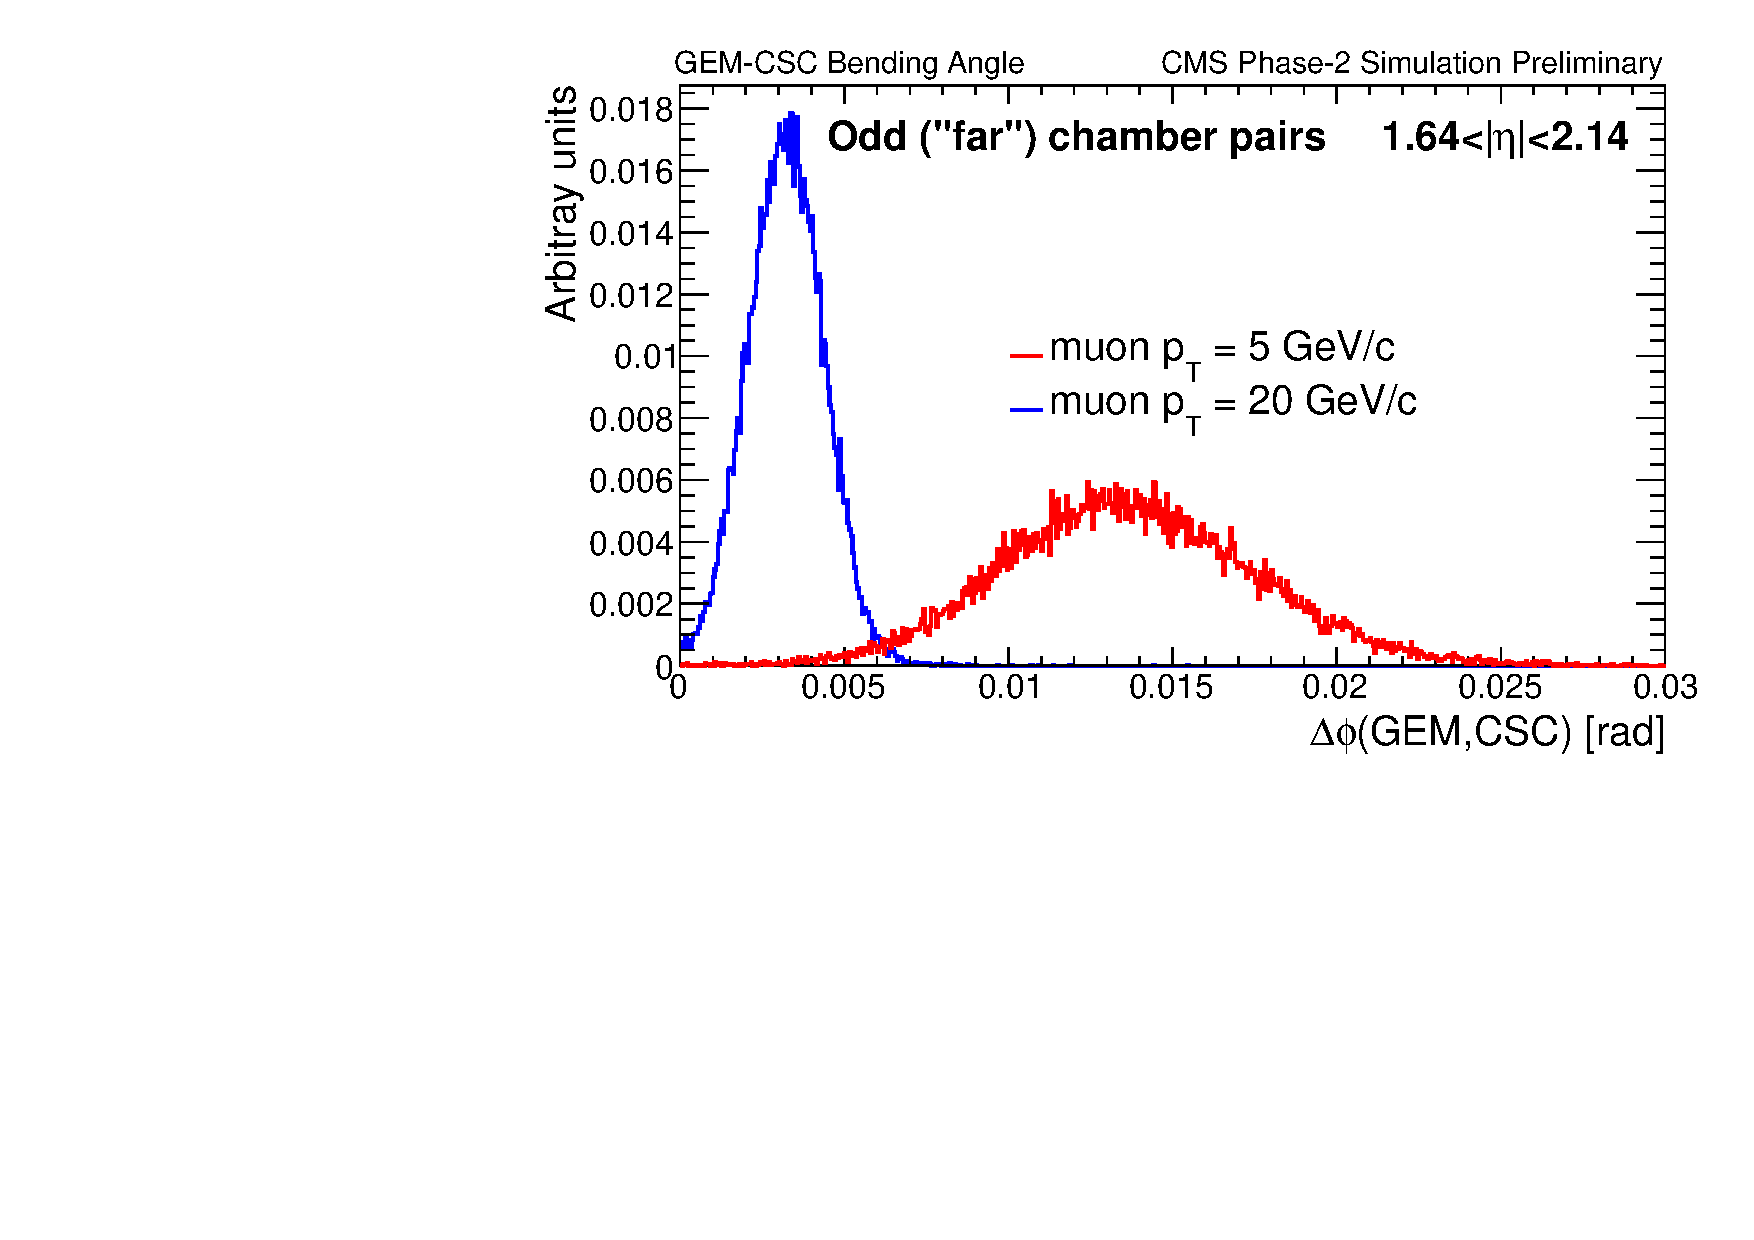
\includegraphics[width=0.53\textwidth]{img/II-1-gem/gem-csc-bending-2.pdf}
      \caption{Left: sketch of the measurement of the bending angle with a pair of CSC and GEM chambers, illustrating the difference between lower and higher momentum muons. Right: $ \Delta \phi = \phi_{GE1/1} - \phi_{ME1/1} $ distribution for 5 GeV/c and 20 GeV/c p$_T$ muons demonstrating the discrimination power of the combined GEM-CSC system \cite{Colaleo:2021453}.}
      \label{fig:II-1-csc-bending}
    \end{figure}

    Using these results, a common effort from the GEM and CSC collaborations ensued to integrate the GEM measurements in the CSC trigger system to provide an additional layer of information. By the means of simulations, it has been shown that the efficiency of the combined system increases, thus yielding a lower rate of fake triggers. These results are shown in Figure \ref{fig:II-1-trigger}. In the left plot, which shows the efficiency as a function of the pseudorapidity of the particles, it can be seen that the efficiency of the GEM and CSC combined trigger (blue) is superior to the CSC only results (red), recovering the losses occurring at higher rates. In the right plot which shows the trigger rate as a function of the cut applied on the momentum of the particle, it is depicted how the trigger rate of the combined system (blue) diminishes by one order of magnitude compared to the current system (red). For a given trigger rate, a smaller muon p$_T$ threshold can be applied due to the lower rate of misreconstructed particles, which improves the performance of the detectors. \\

    \begin{figure}[t!]
      \centering
      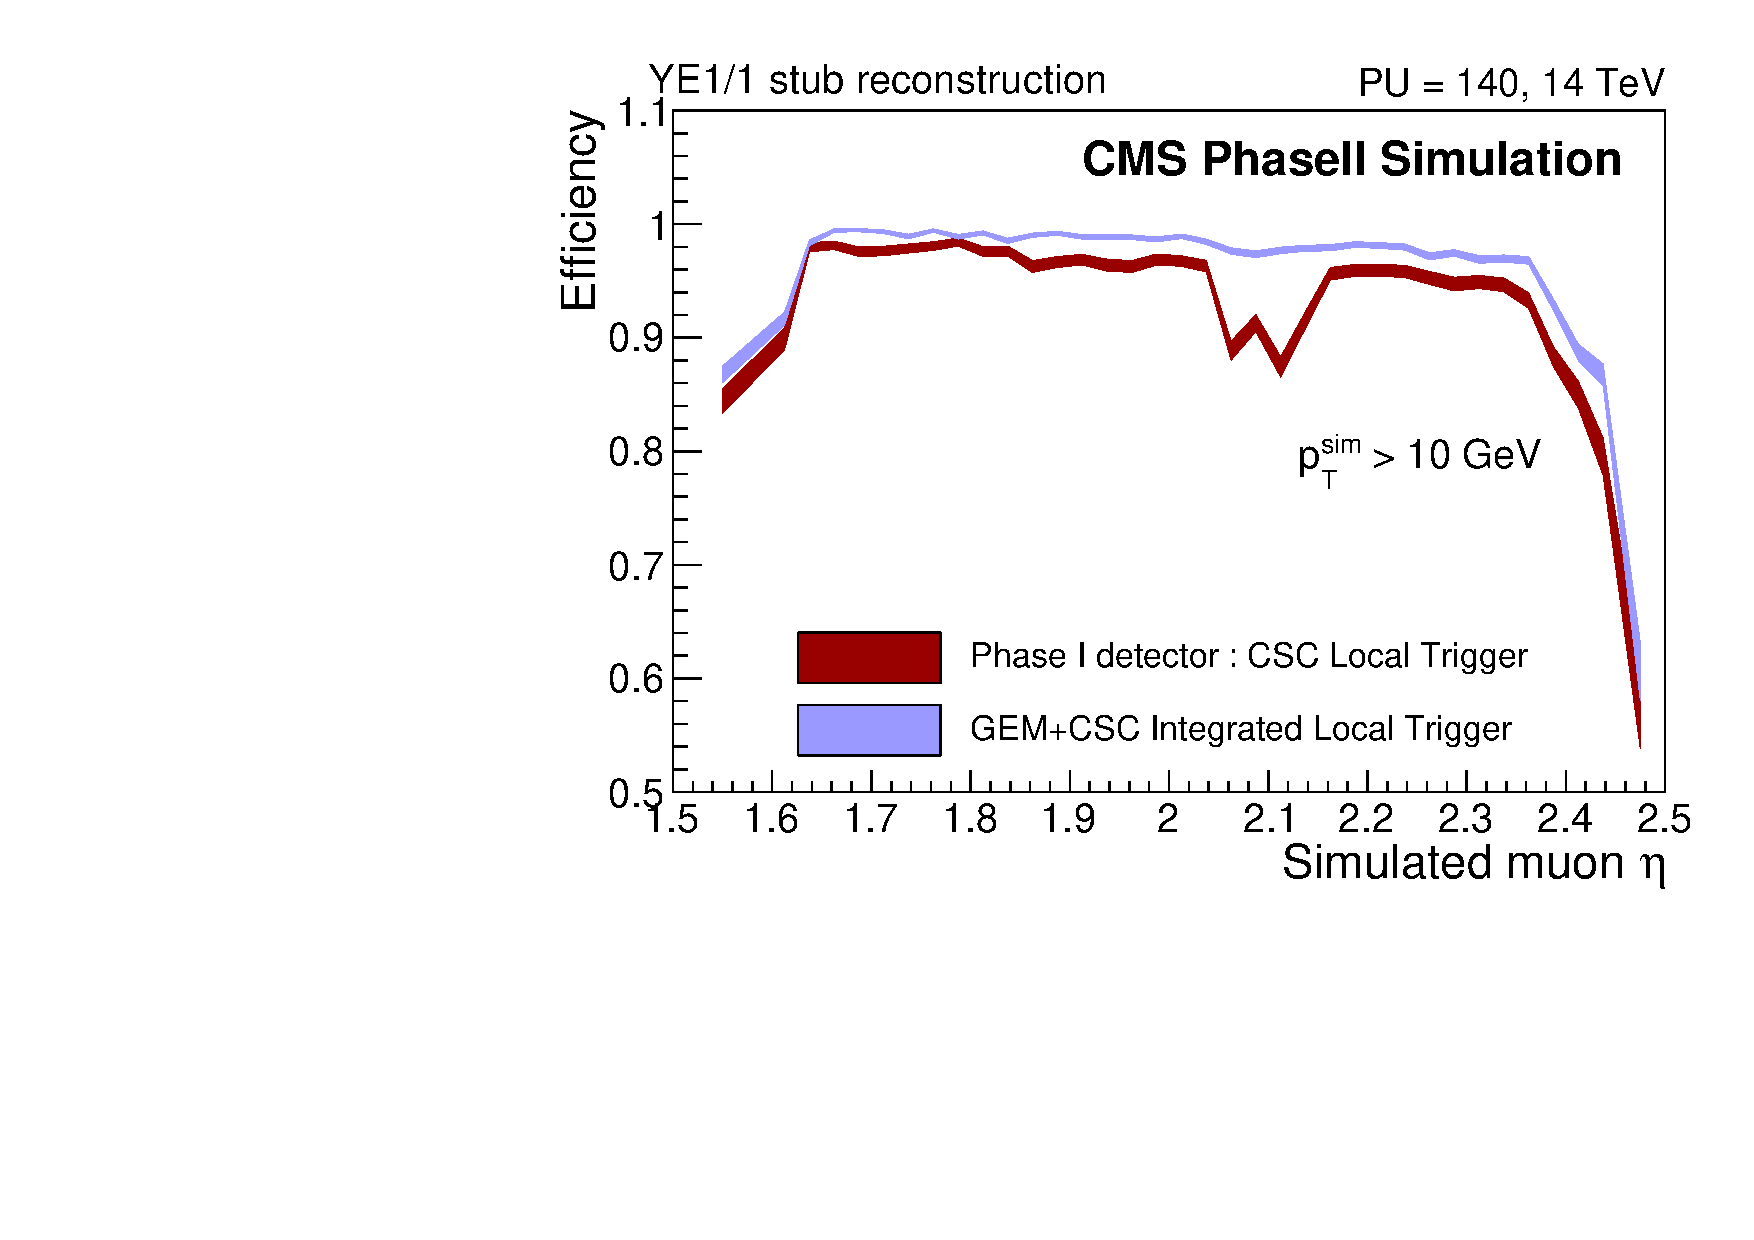
\includegraphics[width=\textwidth]{img/II-1-gem/gem-csc-efficiency.pdf}
      \caption{Left: reconstruction efficiency of the integrated GEM-CSC trigger as a function of the simulated muon |$\eta$|, compared to the same for the Phase-I CSC-only algorithm. Right: level 1 muon trigger rates before and after the GE1/1 upgrade at a luminosity of 2 $\times$ 10$^{34}$ cm$^{-2}$ s$^{-1}$. MS1/1 denotes the first endcap muon station level 1 trigger in both cases, i.e. with CSC-only or with the combination CSC and GEM trigger information \cite{Colaleo:2021453}.}
      \label{fig:II-1-trigger}
    \end{figure}

    Preserving a low p$_T$ threshold is essential for physics analysis to yield a reliable reconstruction efficiency for soft muons, that is muons with low momentum. These particles are important for a wide range of processes from beyond the Standard Model searches to measurements in the Higgs sector. Simulation studies have shown that in the case of $ H \rightarrow \tau^+ \tau^- $ where one $ \tau $ decays into a muon and the other hadronically, a decrease of 5 GeV in the p$_T$ threshold results in an increase of 35\% in the acceptance of the channel. In addition, the impact is not limited to the single muon trigger but affects all other triggers involving muons analysis, for example, $\mu+jet$ or $e/\gamma+\mu$ signals. \\

    To further improve the trigger efficiency of CMS, it is planned to integrate a new track trigger, a trigger system for the tracker, which would benefit from the high resolution of the silicon subdetector. Foreseen to be installed during LS3, the system yields excellent results in the identification, reconstruction, and triggering of muons. However, due to the high occupancy of hits and the limited amount of computational time allocated to the trigger, given approximations must be done, degrading the results for certain physics channels. One of the assumptions made by the algorithms is that every particle originates from the interaction point. This has a significant impact on new physics processes involving hidden sectors of low interacting particles such as the decay of a Higgs into two neutralinos $ n_1 $, which in turn create a dark photon $ \gamma_d $
    \begin{equation}
      h \rightarrow 2 n_1 \rightarrow 2 n_d \gamma_d .
    \end{equation}
    The dark photon in turn decays into two muons which originate from a displaced vertex. Figure \ref{fig:II-1-dark-photon} illustrates the limitations of the track trigger (red) to reconstruct muons as a function of the distance between the vertex and the interaction point. Efficiency quickly drops to reach 0\% around 50 cm. The muon standalone trigger (blue) on the other hand is capable of reconstructing the track with high efficiency underlining the necessity of preserving excellent trigger performances in the muon spectrometer.

    \begin{figure}[t!]
      \centering
      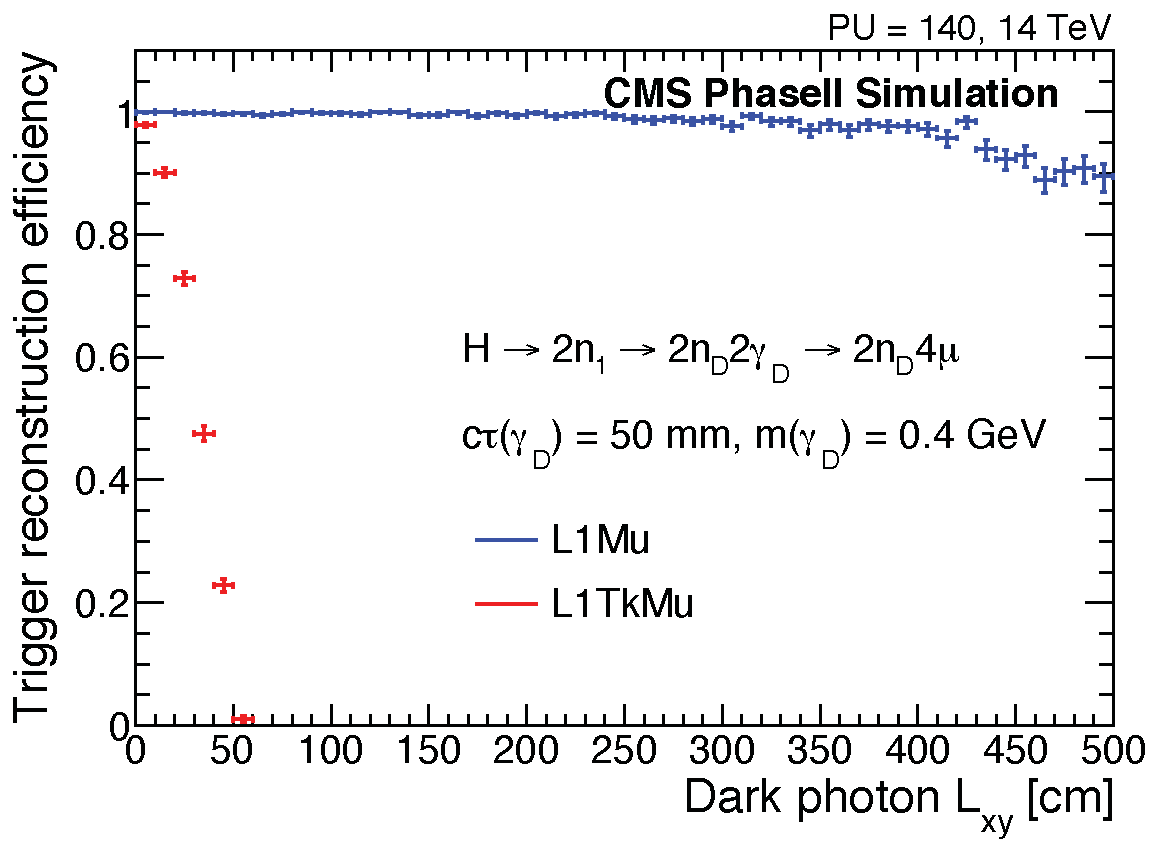
\includegraphics[width=0.6\textwidth]{img/II-1-gem/dark-photon.pdf}
      \caption{The probability of reconstructing at least one muon candidate produced in the decay of a light long-lived particle decaying to a pair of muons $\gamma_d \rightarrow \mu \mu $ as a function of L$_{xy}$, the distance between the $\gamma_d$ decay vertex to the beamline in the transverse plane. Standalone muon trigger L1Mu performance is compared to that of L1TrkMu, a trigger based on matching muon and track trigger candidates with the CMS Phase-II detector simulation \cite{Colaleo:2021453}.}
      \label{fig:II-1-dark-photon}
    \end{figure}

  \section{Technology Overview of Triple-GEM detectors}

    A GEM foil is a 50-$\mu$m-thick polymer foil covered with 5-$\mu$m-thin copper sheets on both sides, and chemically perforated by a high density of microscopic holes. The polymer used is either Kapton or Apical, both with a dielectric constant of 3.5. The holes are truncated double cones with an outer diameter of 70 $\mu$m and a inner diameter of 50 $\mu$m and are spaced by 140 $\mu$m on an hexagonal grid. The structure of the GEM foil as shown on the left in Figure \ref{fig:II-1-holes}, is obtained using photolitography techniques that require precise alignment of the top and bottom masks. \\

    The diagram on the right in Figure \ref{fig:II-1-holes} represents the electric field lines that appear when a high voltage difference is applied between the two layers of copper, typically on the order of 300 V, resulting in field densities inside the holes reaching approximately 80 kV cm$^{-1}$. The structure of the electric field is used to amplify the signal of particles passing through the detector. Electrons resulting from the ionization of the gas by charged particles are directed towards the holes of the foil. When reaching high kinetic energy inside the holes, they themselves ionize the medium, producing secondary avalanches of electrons. Each hole acts as a proportional counter with gains up to 800 at voltages between 500 and 550 V.  \\

    \begin{figure}[h!]
      \centering
      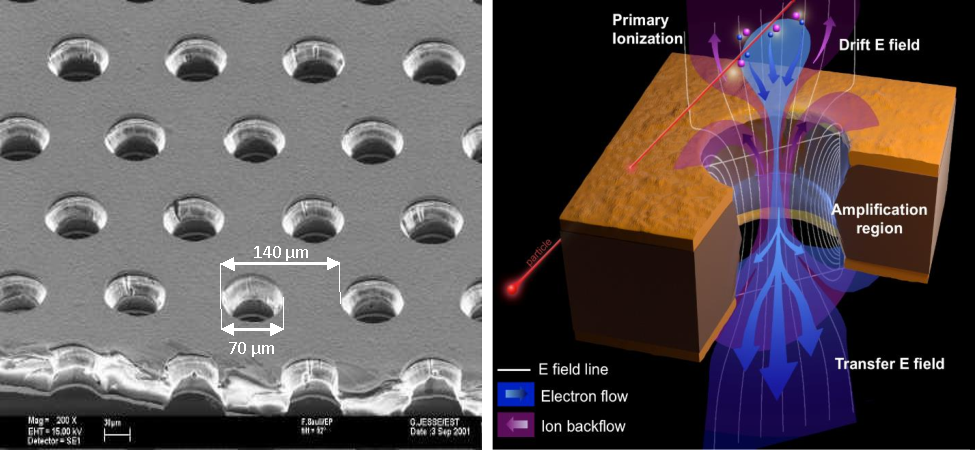
\includegraphics[width=\textwidth]{img/II-1-gem/holes.pdf}
      \caption{Left: scanning electron microscope picture of a GEM foil. Right: schematic view of the electric field lines (white), electron flow (blue), and ion flow (purple) through a bi-conical GEM hole \cite{Colaleo:2021453}.}
      \label{fig:II-1-holes}
    \end{figure}

    To achieve high gains in the detectors, two solutions can be implemented: increase the high voltage on the foils, or use multiple foils. The first option gives rise to discharges when operating at too high electric fields thus damaging the detector. Therefore, the choice to use three GEM foils has been made, hence the name of Triple-GEM detectors. The foils are arranged as shown in Figure \ref{fig:II-1-triple} which depicts the principle of operation of a triple-GEM chamber. A drift cathode is placed on the top of the chamber which creates an electric field between itself and the top copper layer of the first GEM foil in the so-called drift gap measuring 3 mm. Electrons originating from the ionization of the gas mixture (either 70\% Argon + 30\% CO$_2$ or 45\% Argon + 15\% CO$_2$ + 40\% CF$_4$) by a charged particle drift towards the holes of the foil, while ions are collected by the cathode. Following, the electron shower is amplified by GEM 1, GEM 2, and GEM 3, respectively transferring the signal to the transfer 1, transfer 2, and induction gaps measuring 1 mm, 2 mm, and 1 mm respectively. The size of each gap is of importance in the detector performance and has been optimized over time to increase the speed of the signal and the efficiency. The current configuration is called 3/1/2/1 mm in reference to the gap size. In the induction gap, the drift of the electrons towards the anodes induces a signal on the latter which can be detected by electronics. The choice to use either ArCO$_2$ or ArCO$_2$CF$_4$ has yet to be made. Although the use of CF$_4$ improves given parameters of the detector exposed bellow, CMS has limited its use due to its toxicity for the environment. \\

    \begin{figure}[t!]
      \centering
      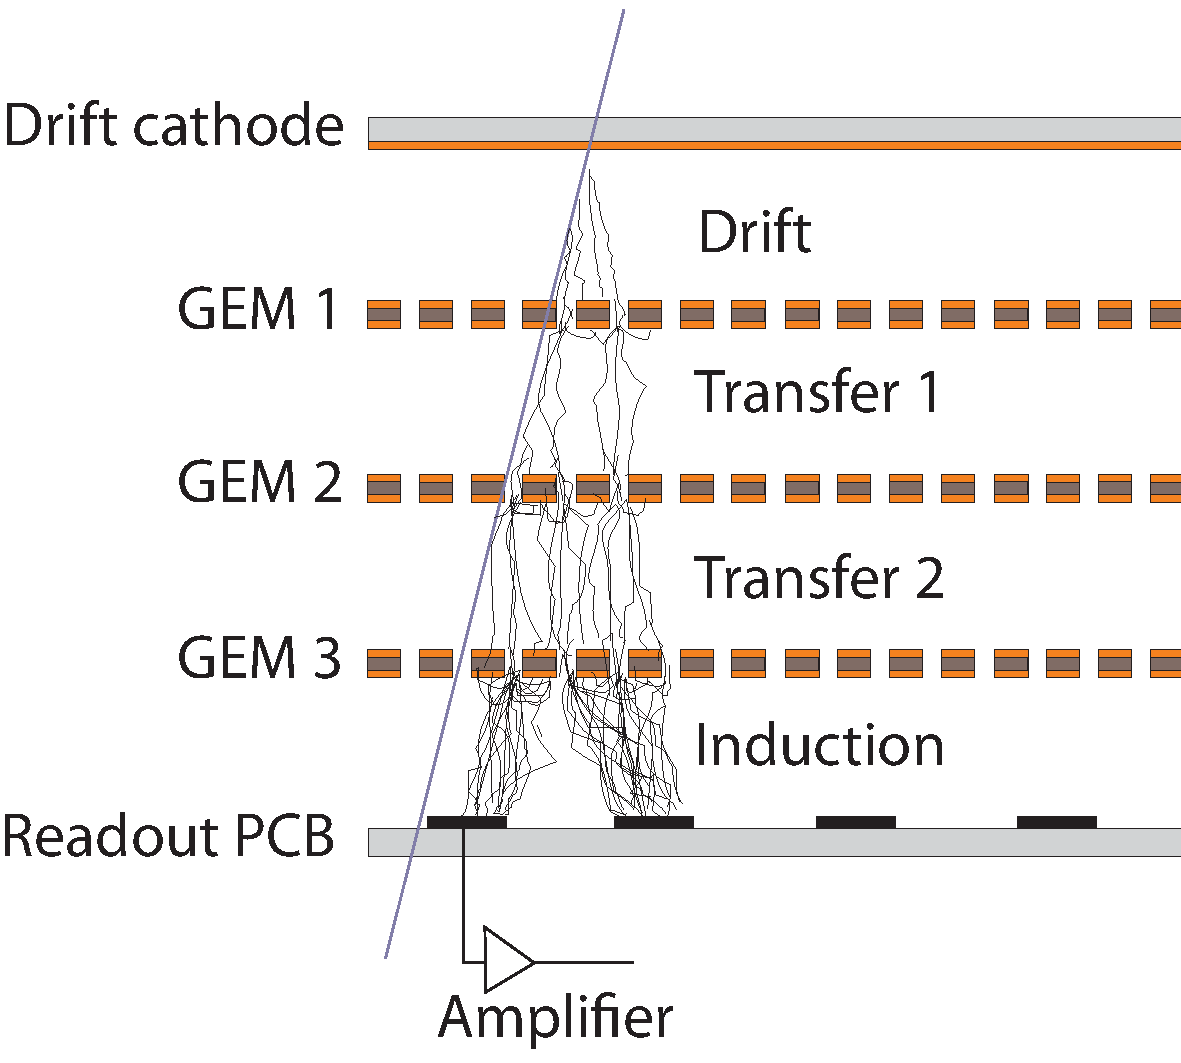
\includegraphics[width=0.7\textwidth]{img/II-1-gem/triple-gem-foils.pdf}
      \caption{Principle of operation of a generic triple-GEM chamber and definition of drift, transfer, and signal induction gap regions within the detector \cite{Colaleo:2021453}.}
      \label{fig:II-1-triple}
    \end{figure}

  \section{Technical Design of GE1/1 chambers for CMS}

    The GE1/1 chambers are arranged in pairs to form superchambers, each covering 10$^o$ in $ \phi $ for a total of 72 chambers per endcap. Figure \ref{fig:II-1-superchamber} displays the geometry of the superchambers. Due to mechanical constraints, the trapezoidal chambers are declined in two versions: a short one and a long one. The short chambers cover 1.61 < |$\eta$| < 2.18 and have a large base of 445 mm, a small base of 220 mm, and a height of 990 mm. The long chambers cover 1.55 < |$\eta$| < 2.18 and have a large base of 510 mm, a small base of 279 mm, and a height of 1283 mm. \\

    \begin{figure}[b!]
      \centering
      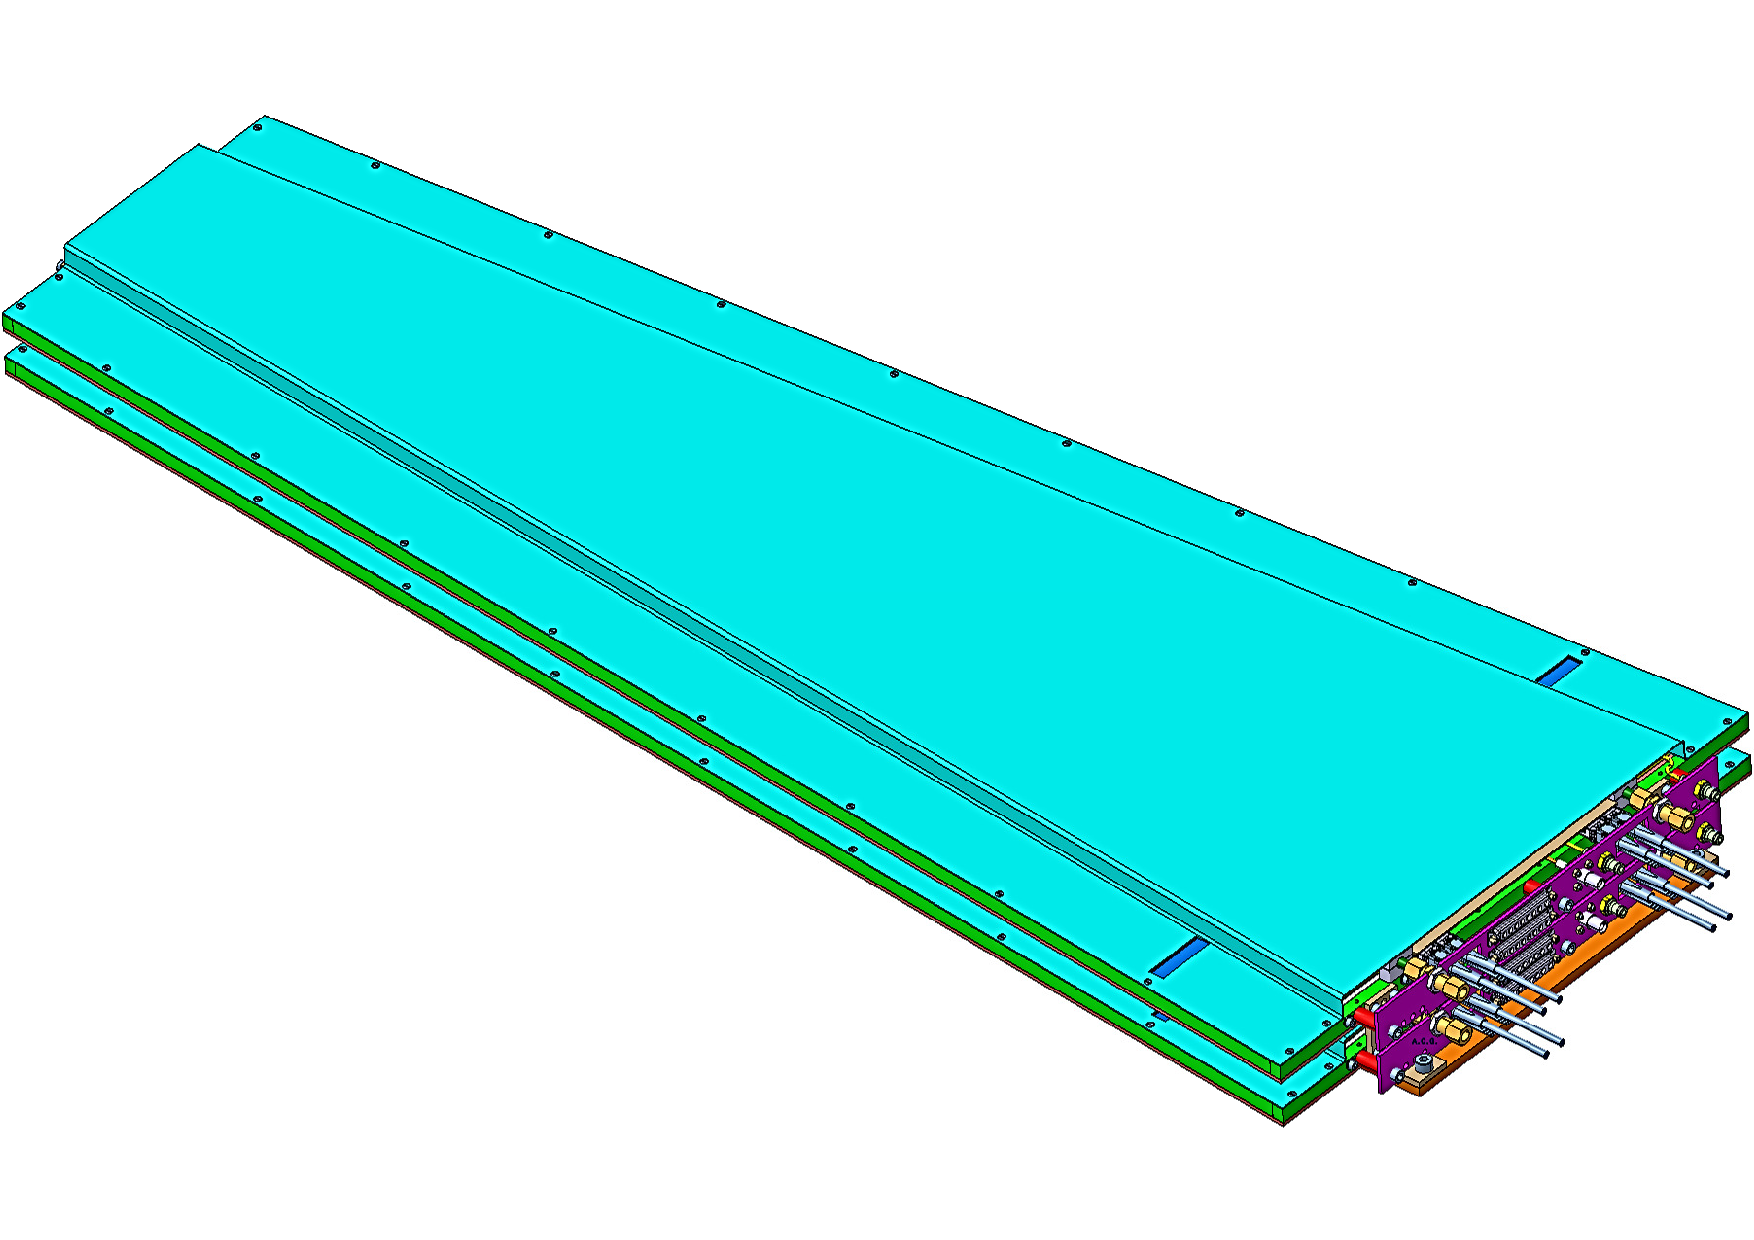
\includegraphics[width=0.7\textwidth]{img/II-1-gem/superchamber.pdf}
      \caption{A pair of GEM chambers form a superchamber \cite{Colaleo:2021453}.}
      \label{fig:II-1-superchamber}
    \end{figure}

    The structure of a single chamber is shown in Figure \ref{fig:II-1-exploded} which provides an exploded view of the detector. The drift cathode is placed on the bottom of the detector on which a frame is attached. The three GEM foils are stretched out using screws embedded in the frame along with the seals making the chamber air tight. The anode strips are engraved on the readout board that closes the active region of the detector. One chamber is divided into three $ \phi $ sectors and eight $ \eta $ sectors with 128 strips running radially in each. This results in a mean coverage per strip of 450 $\mu$rad and a pitch varying from approximately 500 $\mu$m to 1.3 mm. To each group of 128-strips a front-end electronics chip called the VFAT3 is attached. This chip digitizes the signals from the strips returning a single hit/not-hit bit. The VFAT3s are all connected to the GEM electronics board which acts as router to forward the data towards the OptoHybrid, a concentrator board located on the large side of the GEM which is the interface to the off-detector electronics. The VFAT3s and the OptoHybrid are cooled down using cooling pipes attached on the top of the boards. Finally, a protective cover closes and protects the detector. When two chambers are assembled, a patch panel is added in order to facilitate the insertion and removal of the low and high voltage cables, the water for the cooling, the gas, and the optical fibers connected to the DAQ system. Note that a single source of high voltage is needed to power a chamber thanks to the use of a ceramic voltage divider which spreads the voltage over the various layers. \\

    \begin{figure}[t!]
      \centering
      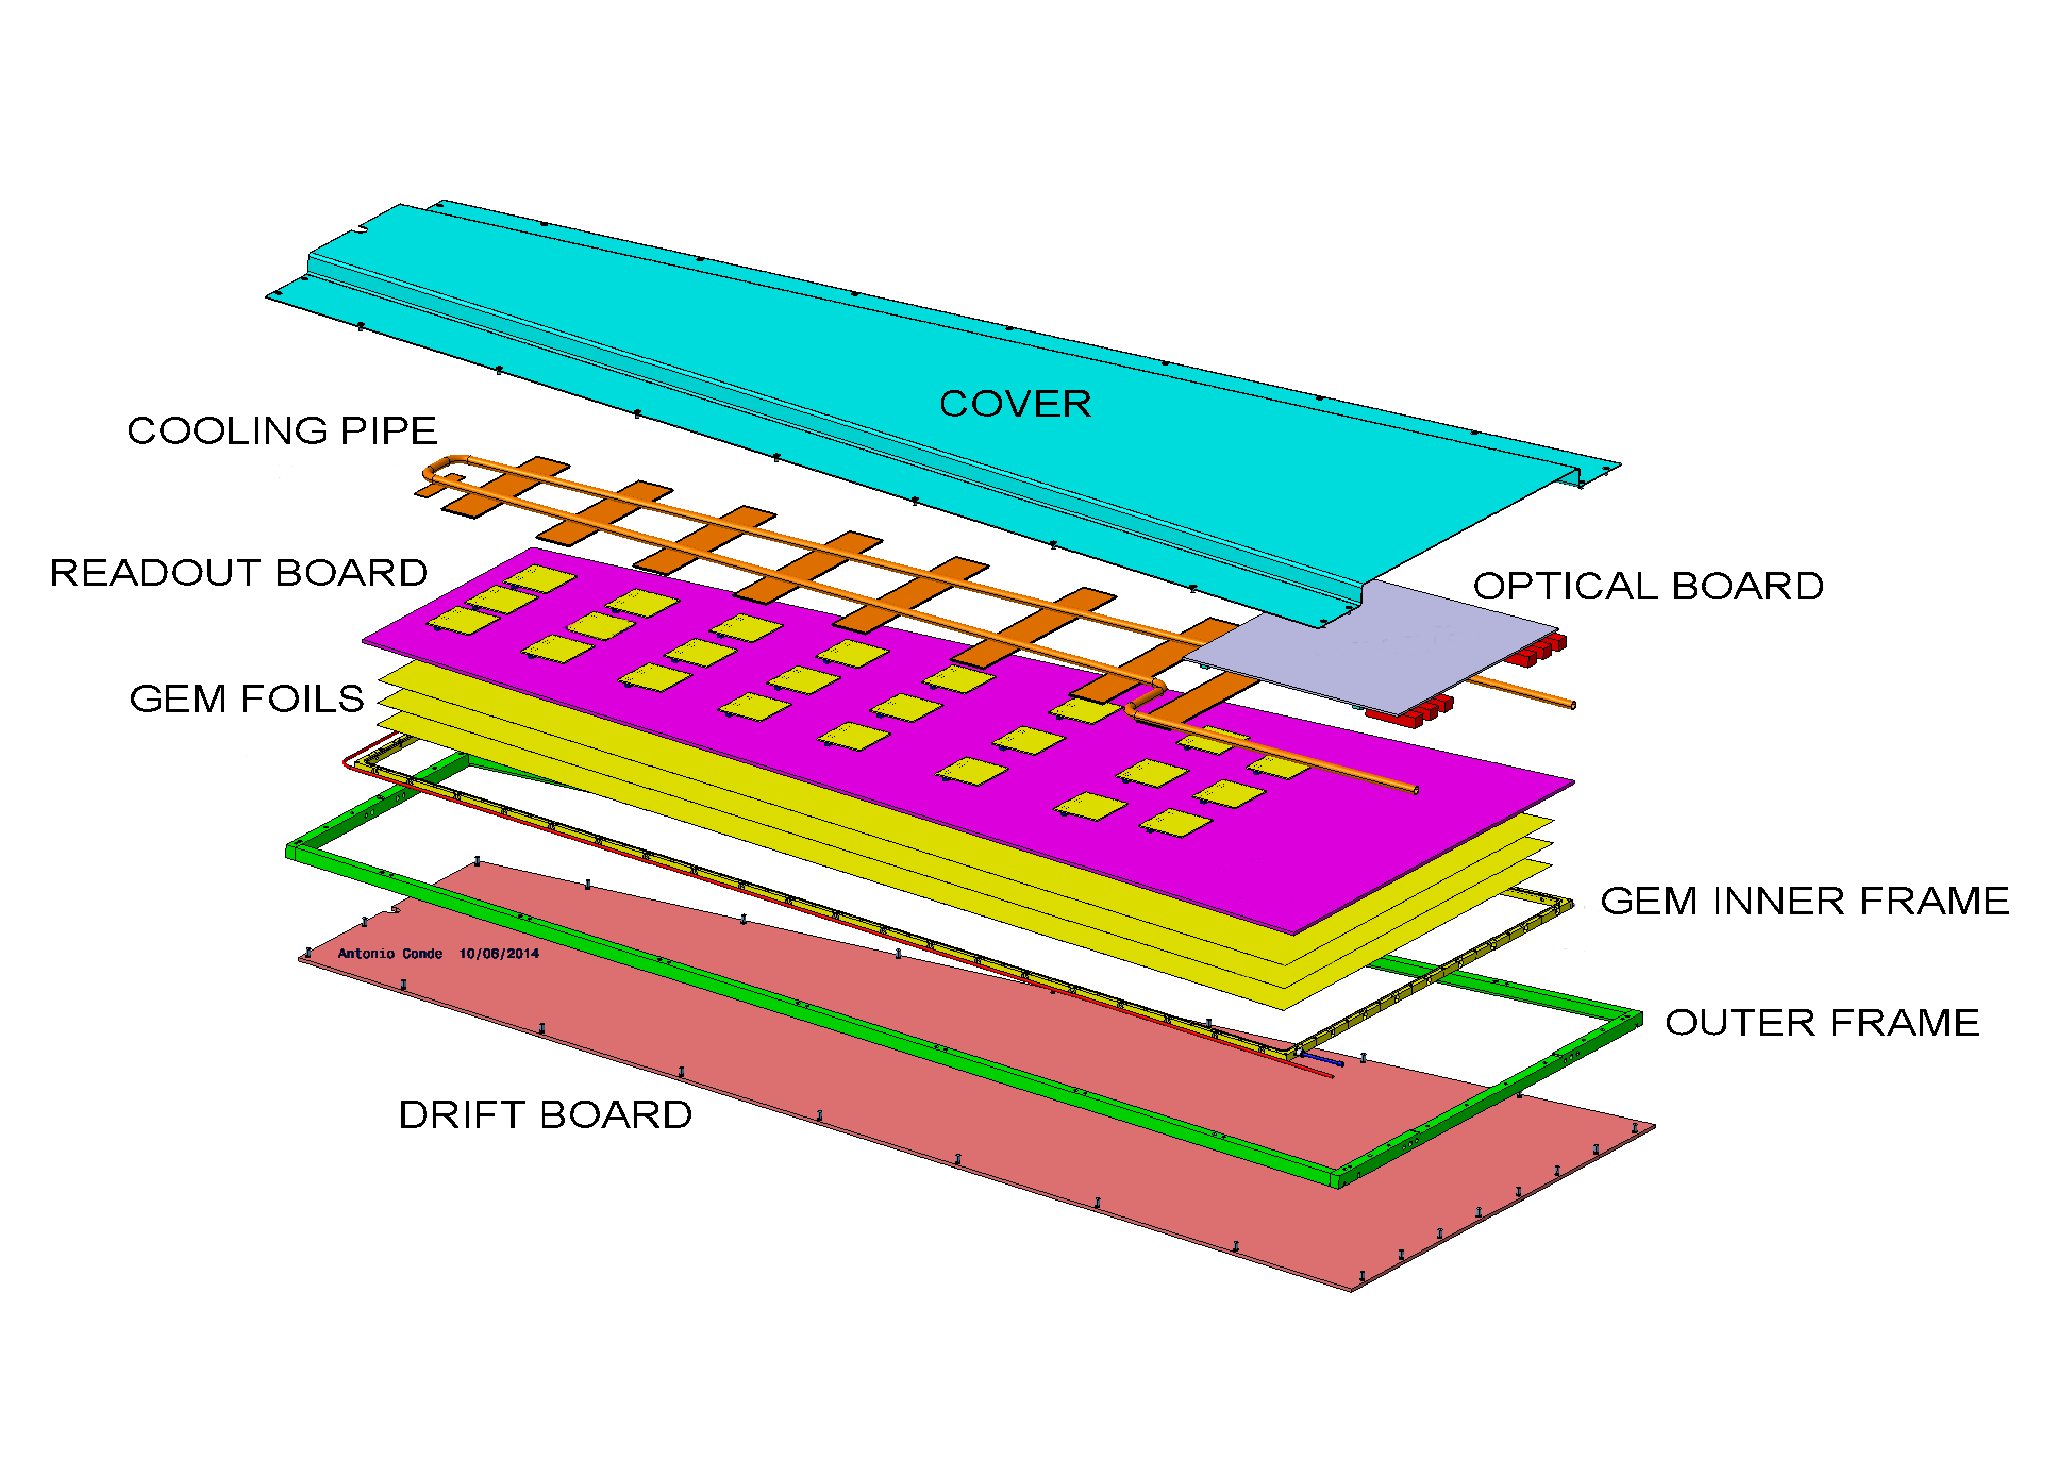
\includegraphics[width=\textwidth]{img/II-1-gem/gem-exploded.pdf}
      \caption{Exploded view of the mechanical design of a Triple-GEM chamber \cite{Colaleo:2021453}.}
      \label{fig:II-1-exploded}
    \end{figure}

    Once assembled, the 72 superchambers will be installed in the endcaps of CMS as displayed in Figure \ref{fig:II-1-wheel} showing the first station of the endcap of CMS. The full ring will be placed in the so-called nose of the endcap, between the HCAL and the ME1/1 CSC stations.

    \begin{figure}[p]
      \centering
      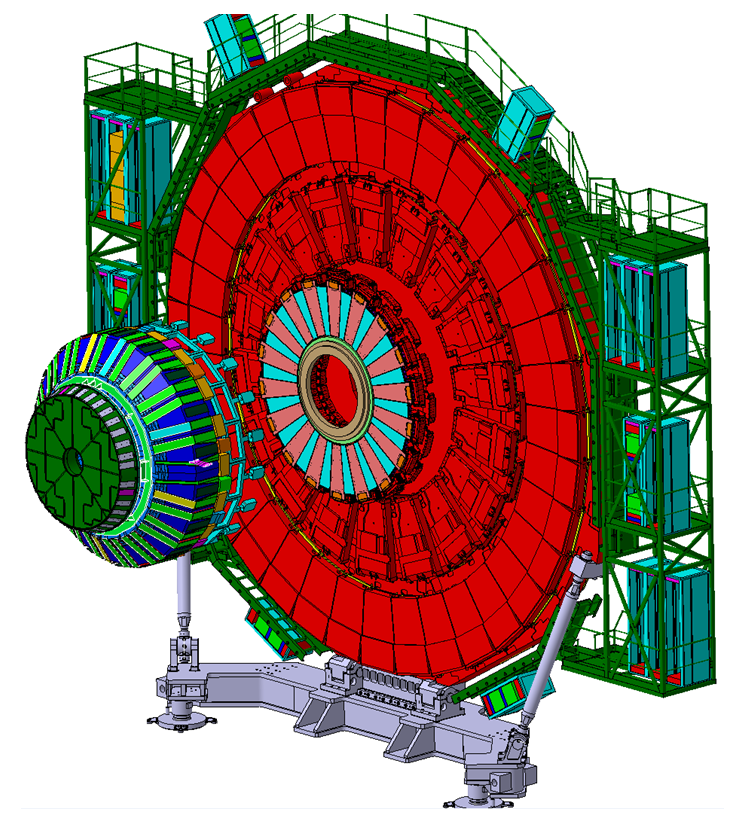
\includegraphics[width=\textwidth]{img/II-1-gem/wheel.png}
      \caption{First CMS muon endcap station where the inner ring is equipped with 18 long (red) and 18 short (blue) triple GEM superchambers \cite{Colaleo:2021453}.}
      \label{fig:II-1-wheel}
    \end{figure}

  \section{Detector Design Evolution}

    The design and fabrication method of the GE1/1 chambers has evolved over the past five years of R\&D. Figure \ref{fig:II-1-generations} shows the five generations of detectors that have been developed. GE1/1-I was the first 1-m-long prototype. It was equipped with only eight readout sectors, components were glued together, and GEM foils were separated using spacers. The number of sectors was increased to 24 in GE1/1-II with the full granularity of the current design (384 strips per 10$^o$). The gap configuration was changed from 3/2/2/2 mm to 3/1/2/1 mm to increase the signal speed. From GE1/1-III and onwards, GEM foils were stretched mechanically using an outer frame glued on the drift board. This design also introduced the use of a miniature ceramic high-voltage divider to apply voltage on the foils. However, the assembly of the chamber induced mechanical tension on the readout board, deforming the detector and resulting in a non-uniform response. This problem was resolved in GE1/1-IV by pre-bending the boards in the opposite direction in order to compensate before being bolted to the frames. This generation was the first assembled without glue, reducing production time to a few hours. However, the pre-beding technique did not yield viable results. Therefore, GE1/1-V uses pull-out pieces to add tension to the foils from the outer frame, on which the drift and readout board are bolted. The outer frame serves as a wall for the chamber and seals it using O-rings. Finally, the version of the design of the chambers that will be installed in CMS is GE1/1-VI which has optimized dimension to maximize the geometrical acceptance.

    \begin{figure}[t!]
      \centering
      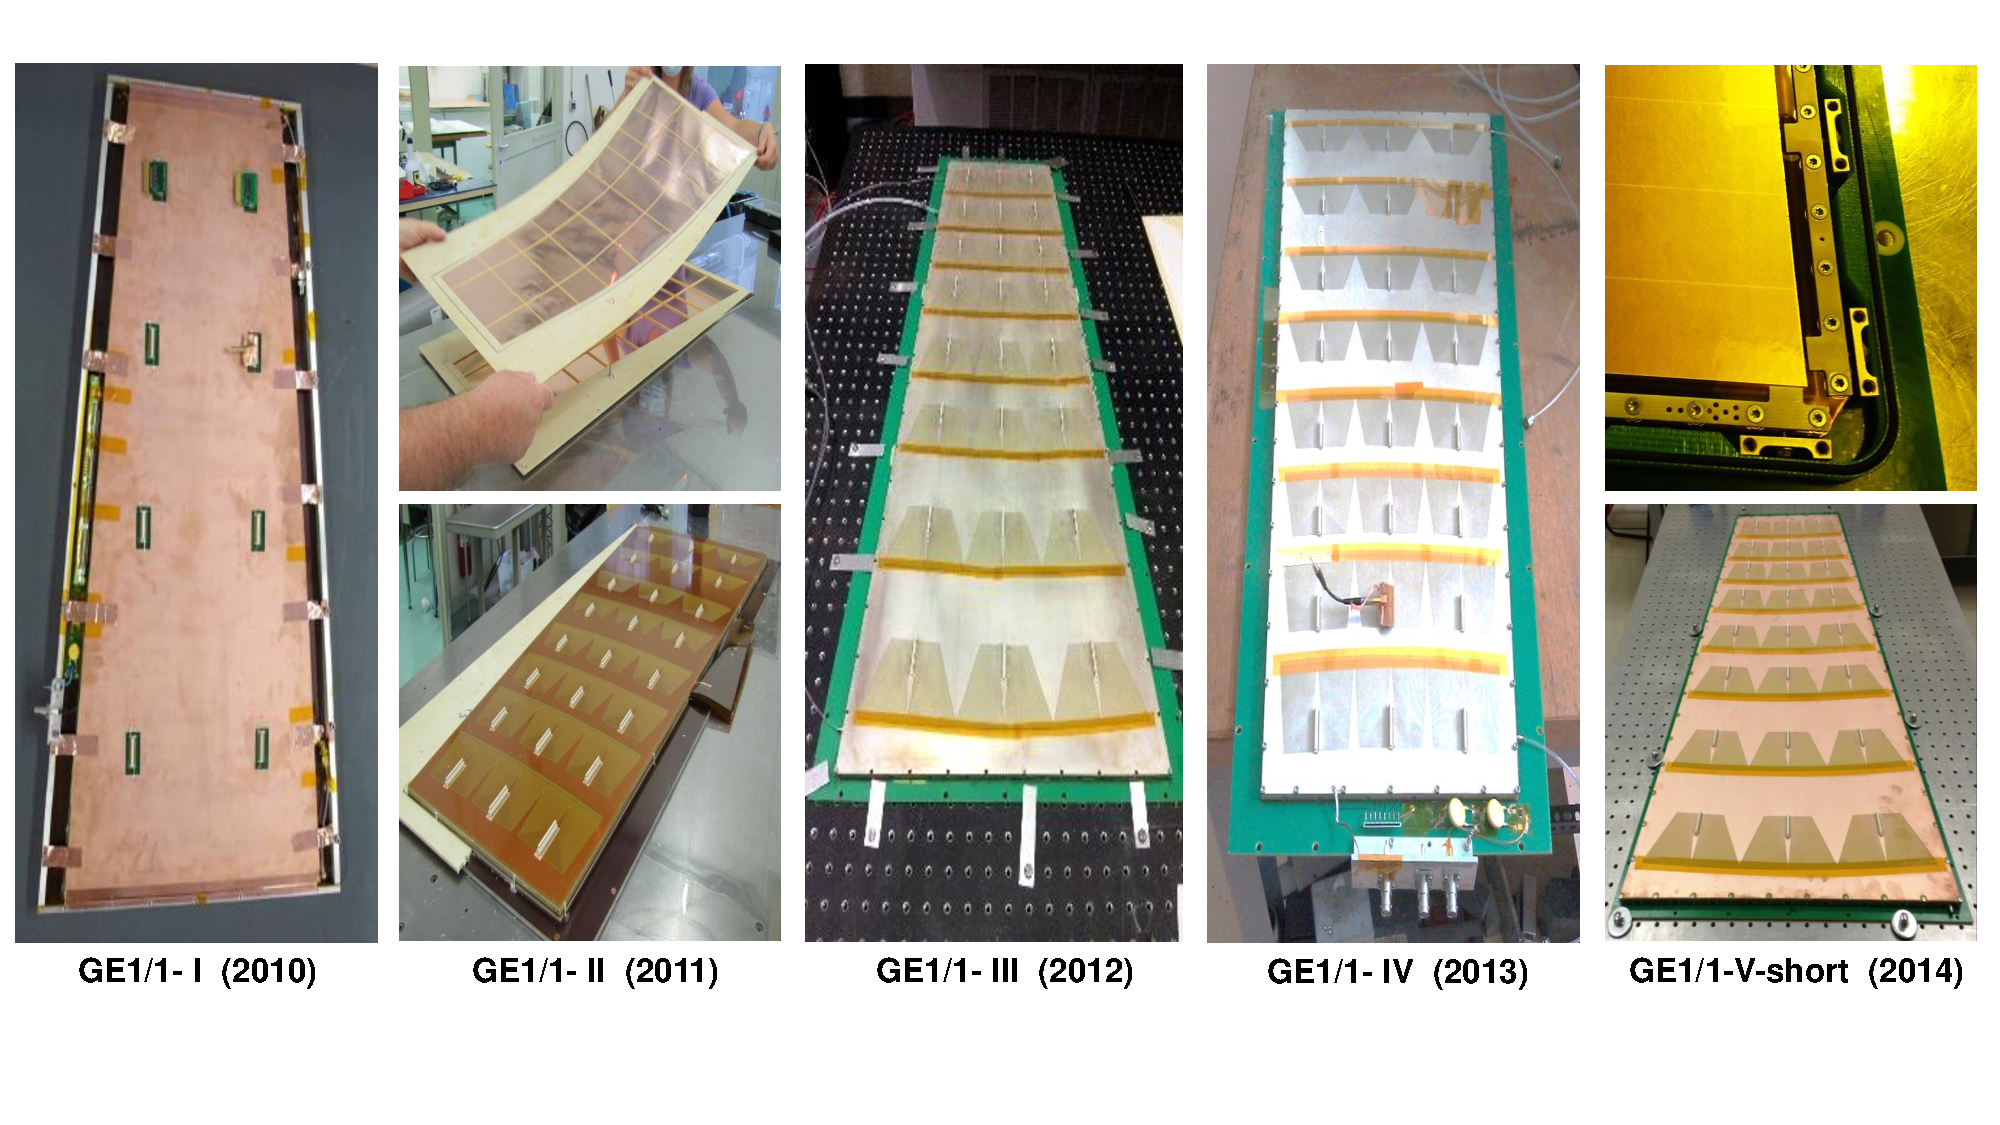
\includegraphics[width=\textwidth]{img/II-1-gem/generations.pdf}
      \caption{Five generations of GE1/1 prototype chambers constructed and tested by the GEM collaboration in 2010-2014. The split figures for GE1/1-II and GE1/1-V demonstrate the evolution from construction using spacer frames to purely mechanical stretching of GEM foils without any spacers \cite{Colaleo:2021453}.}
      \label{fig:II-1-generations}
    \end{figure}

  \section{GE1/1 Prototyping Results}

    In order to provide the desired trigger and physics performance, the GE1/1 chambers must meet the following list of requirements:
    \begin{itemize}
      \item Maximum geometric acceptance within the given CMS envelope;
      \item Rate capability of 10 kHz cm$^{-2}$ or better to cope with the HL-LHC hit rate;
      \item Single-chamber efficiency of 97\% or better for detecting minimum ionizing particles resulting in 99.9\% efficiency for a superchamber when signals are combined with a logical OR;
      \item Angular resolution of 300 $\mu$rad or better on $ \phi_{GE1/1} $ to discriminate high-p$_T$ from low-p$_T$ muons when combining the measurements with ME1/1;
      \item Timing resolution of 10 ns or better for a single chamber, improving when combining the superchamber measurements, to allow matching with the CSC hits;
      \item Gain uniformity of 15\% or better across a chamber and between chambers to ensure that no geometrical or trigger biases are present. \\
    \end{itemize}

    \subsection{Rate Capability}

      Rate capability has been measured by monitoring the gain of a chamber when subject to a 22 keV Ag X-ray source, as represented in Figure \ref{fig:II-1-rate-mes}, and a high-intensity 8 keV Cu source. With ArCO$_2$, gain uniformity is maintained up to 100 MHz cm$^{-2}$, at which point the gain begins to drop. This confirms that the GE1/1 chambers are able to sustain rates up to 10 000 times higher than what they will experience in the 1.6 < |$\eta$| < 2.2 region of CMS. \\

      \begin{figure}[h!]
        \centering
        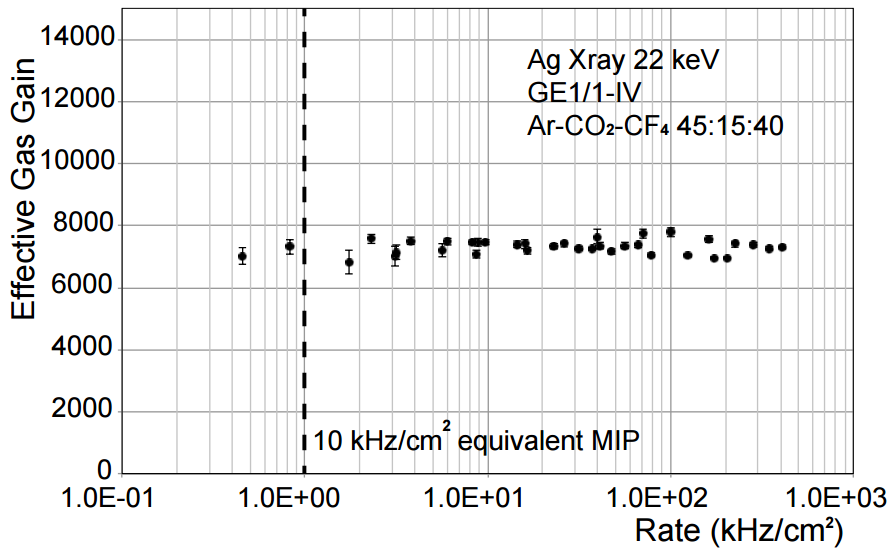
\includegraphics[width=0.9\textwidth]{img/II-1-gem/rate.png}
        \caption{Effective gas gain as a function of the rate of incident particles in a GE1/1-IV detector irradiated with a 22 keV X-ray source \cite{Colaleo:2021453}.}
        \label{fig:II-1-rate-mes}
      \end{figure}

    \subsection{Detection Efficiency}

      The detection efficiency is measured using a multi-layer tracking system placed in front of the detector in a beam of particles. Tracks are reconstructed in the former and extrapolated to the latter to match with reconstructed hits. When using the analog readout electronics, an offline cut is applied on the charge of the strips to cancel noise. In the digital readout system, an online threshold is applied. Figure \ref{fig:II-1-efficiency-hv} plots the evolution of the efficiency as a function of the high voltage applied to the drift electrode for a GE1/1-III chamber operated with ArCO$_2$ at 70\% and 30\% respectively and for different offline cuts on the collected charge. Both results indicate an efficiency plateau at 97\%. \\

      \begin{figure}[t!]
        \centering
        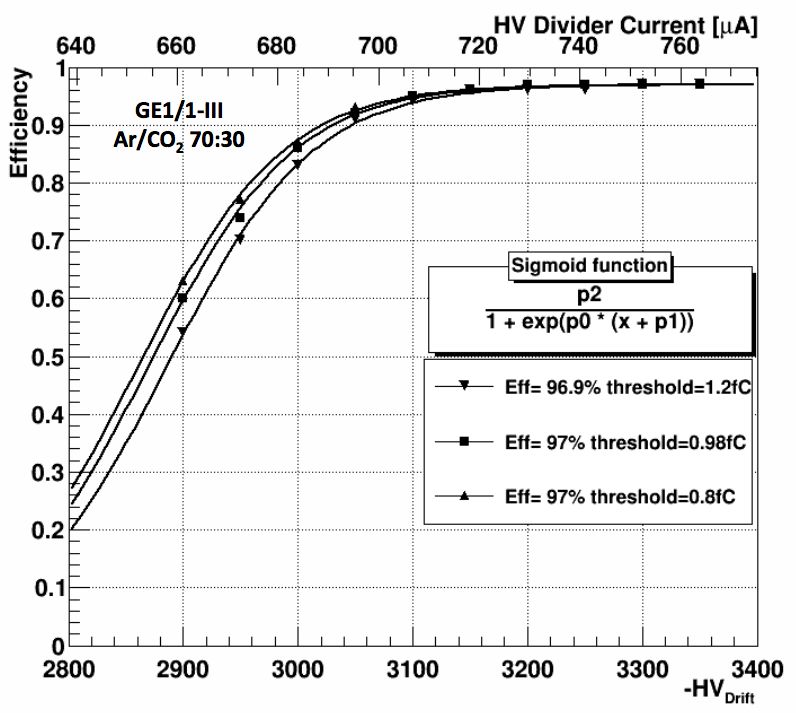
\includegraphics[width=0.85\textwidth]{img/II-1-gem/efficiency.png}
        \caption{Evolution of the efficiency as a function of the high voltage applied to the drift electrode for a GE1/1-III chamber operated with ArCO$_2$ at 70\% and 30\% respectively and for different offline cuts on the collected charge \cite{Colaleo:2021453}.}
        \label{fig:II-1-efficiency-hv}
      \end{figure}

    \subsection{Spatial Resolution}

      Using the above mentioned tracking system, the angular resolution of the GE1/1 chambers has also been measured during test beams. The resolution is taken to be the difference between the projected track position and the measured position in the detector. A resolution of 137$\pm$1 $\mu$rad has been obtained setting an upper limit on the angular resolution which is close to the theoretical value computed for a binary readout of
      \begin{equation}
        \frac{\text{angular strip pitch}}{\sqrt{12}} = \frac{455\  \mu\text{rad}}{\sqrt{12}} = 131\ \mu\text{rad} .
      \end{equation}
      Similar results were obtained using analog readout systems. \\

    \subsection{Time Resolution}

      The timing measurements are done by fitting the spread of the distribution plotting the time difference between a trigger coming from scintillators and the detection of the particle by the GEM detector. Figure \ref{fig:II-1-time-res} shows the time resolution of a small Triple-GEM detector as a function of the electric field in the drift gap. Time resolution studies have been performed using ArCO$_2$CF$_4$ as well as ArCO$_2$ gas mixtures. At the highest voltages, the former yields a resolution of 4 ns due to the fast electron transport speed in CF$_4$ while the latter provides 8 ns \cite{Thierry:2065693}. \\

      \begin{figure}[t!]
        \centering
        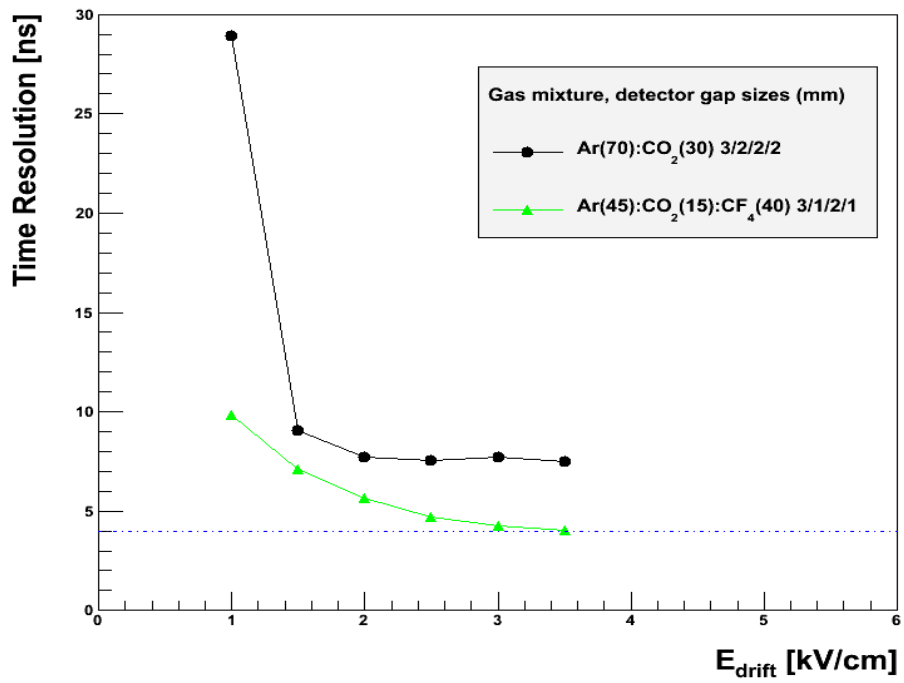
\includegraphics[width=0.8\textwidth]{img/II-1-gem/time-resolution.png}
        \caption{Time resolution of a small Triple-GEM detector as a function of the electric field in the drift gap \cite{Thierry:2065693}.}
        \label{fig:II-1-time-res}
      \end{figure}

    \subsection{Response Uniformity}

      The response uniformity of the GEMs is measured for each detector as part of the quality control process. An X-ray generator is used to scan the entire chamber and the peak amplitude of the pulse charge distribution is taken as measurement of the uniformity. Figure \ref{fig:II-1-uniformity} represents the distribution of the pulse charge measured over different strips on the left, and the evolution of the mean of the distribution of the pulse charge over multiple strips on the right. These tests show that the uniformity of the detector does not vary more than 15\%.

      \begin{figure}[b!]
        \centering
        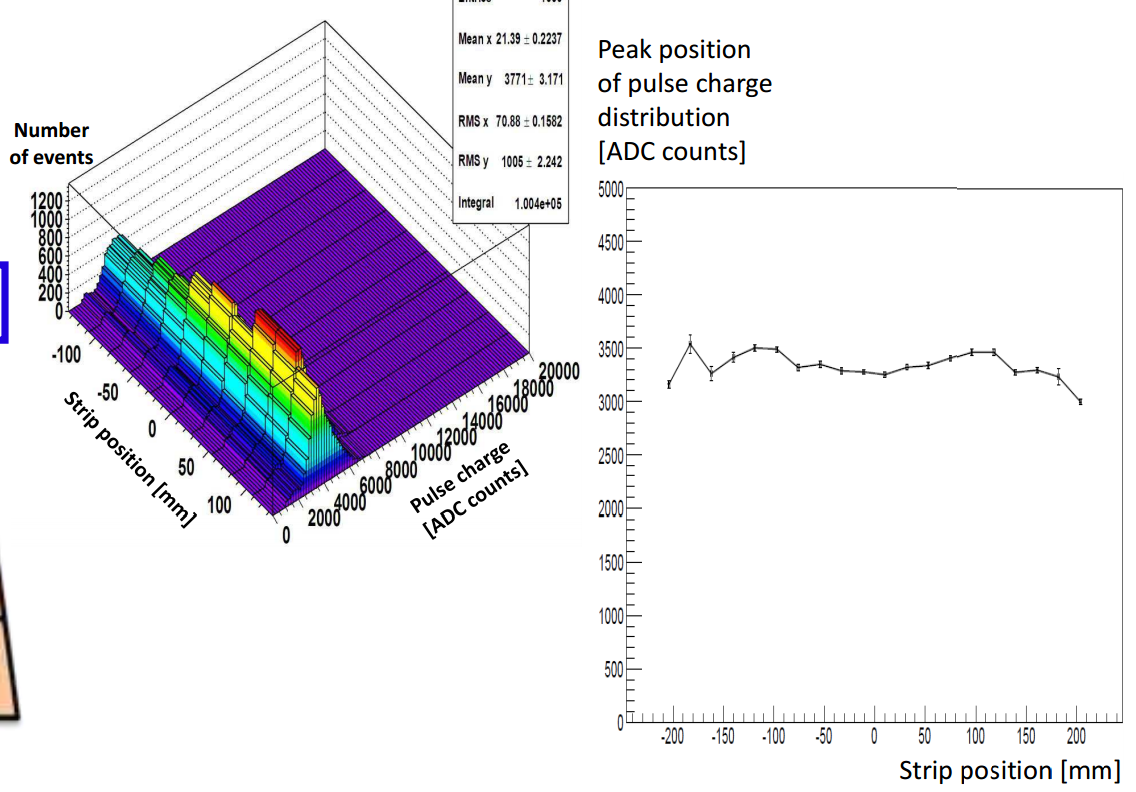
\includegraphics[width=0.9\textwidth]{img/II-1-gem/uniformity.png}
        \caption{Left: distribution of the pulse charge measured over different strips. Right: evolution of the mean of the distribution of the pulse charge over multiple strips \cite{Colaleo:2021453}.}
        \label{fig:II-1-uniformity}
      \end{figure}

  \section{GEM Upgrade Schedule}

    As previously stated, the objective of the GEM collaboration is to install a full ring of GE1/1 detectors in the first muon station of the endcaps during LS2 to maintain good trigger performances. To this end, the collaboration launched a large R\&D program to study the GEM technology and to develop a new DAQ system for the detectors later described in details in Chapter \ref{chap:II-2-daq}. These developments have been and will be tested during test beam campaigns, as well as in CMS to characterize the chambers and prepare the installation in CMS. \\

    Various test beam campaigns have been organized at CERN using the SPS proton beam to produce muons and pions to measure the performance of the detectors and test the developments done on the new DAQ system. The results of the latest test beam are discussed in Chapter \ref{chap:II-3-test-beam}. Besides test beams, mechanical tests have also been operated to prepare the installation of the chambers in the muon spectrometer. At the beginning of LS1, three replicas of superchambers have been installed in CMS to measure the available space and plan for cable space. \\

    At the end of 2016, during the YETS, five superchambers equipped with a full DAQ system will be installed in CMS and connected to the central DAQ of CMS. This small scale test is called the slice test and will demonstrate the integration of the GEMs with the CSCs before the full installation during LS2. As developments on the DAQ systems are still ongoing, the detectors will be equipped with slightly different components in the readout chain. \\

    Finally, before installation in CMS, each component needs to be qualified and characterized, as well as tested against the effects of radiation. To this end, automated procedures have been developed and are described in Chapters \ref{chap:II-4-qualification} and \ref{chap:II-5-irradiation}.

  \section{Developments Beyond GE1/1}

    Next to GE1/1, two other projects are under study by the CMS GEM collaboration: GE2/1 which would instrument the second inner muon station with GEMs, and ME0 which would extend the coverage of the muon spectrometer up to $\eta$ = 3.5. Figure \ref{fig:II-1-ls3} shows a longitudinal view of a quadrant of CMS highlighting the location of the GE1/1, GE2/1, and ME0 detectors colored in red within the muon spectrometer. These projects are still under development and proposed to be installed during LS3, before the start of the LHC Phase II. \\

    The GE2/1 upgrade proposes to install 36 superchambers of Triple-GEM detectors next to the CSCs ME2/1 stations in the 1.60 < |$\eta$| < 2.46 region. Each detector would cover 20$^o$ in $\phi$ and measure 1.84 m in length, 1.18 m in width, and 81 mm in height. Due to the large size of the detectors, they would be segmented in eight $ \eta $ and six $ \phi $ sectors. \\

    The ME0 project aims at installing a 6-layered Triple-GEM detector behind the future shortened HCAL, which upgrade will take place during LS3. This would extend the coverage of the muon spectrometer in the 2.0 < $|\eta|$ < 3.5 region and provide efficient muon identification with low background. The detectors will be subject to high rates of particles, of the order of the MHz cm$^{-2}$, and be exposed to high doses of radiation. The latter will impact the design of the readout electronics and the components that will be selected.

    \begin{figure}[t!]
      \centering
      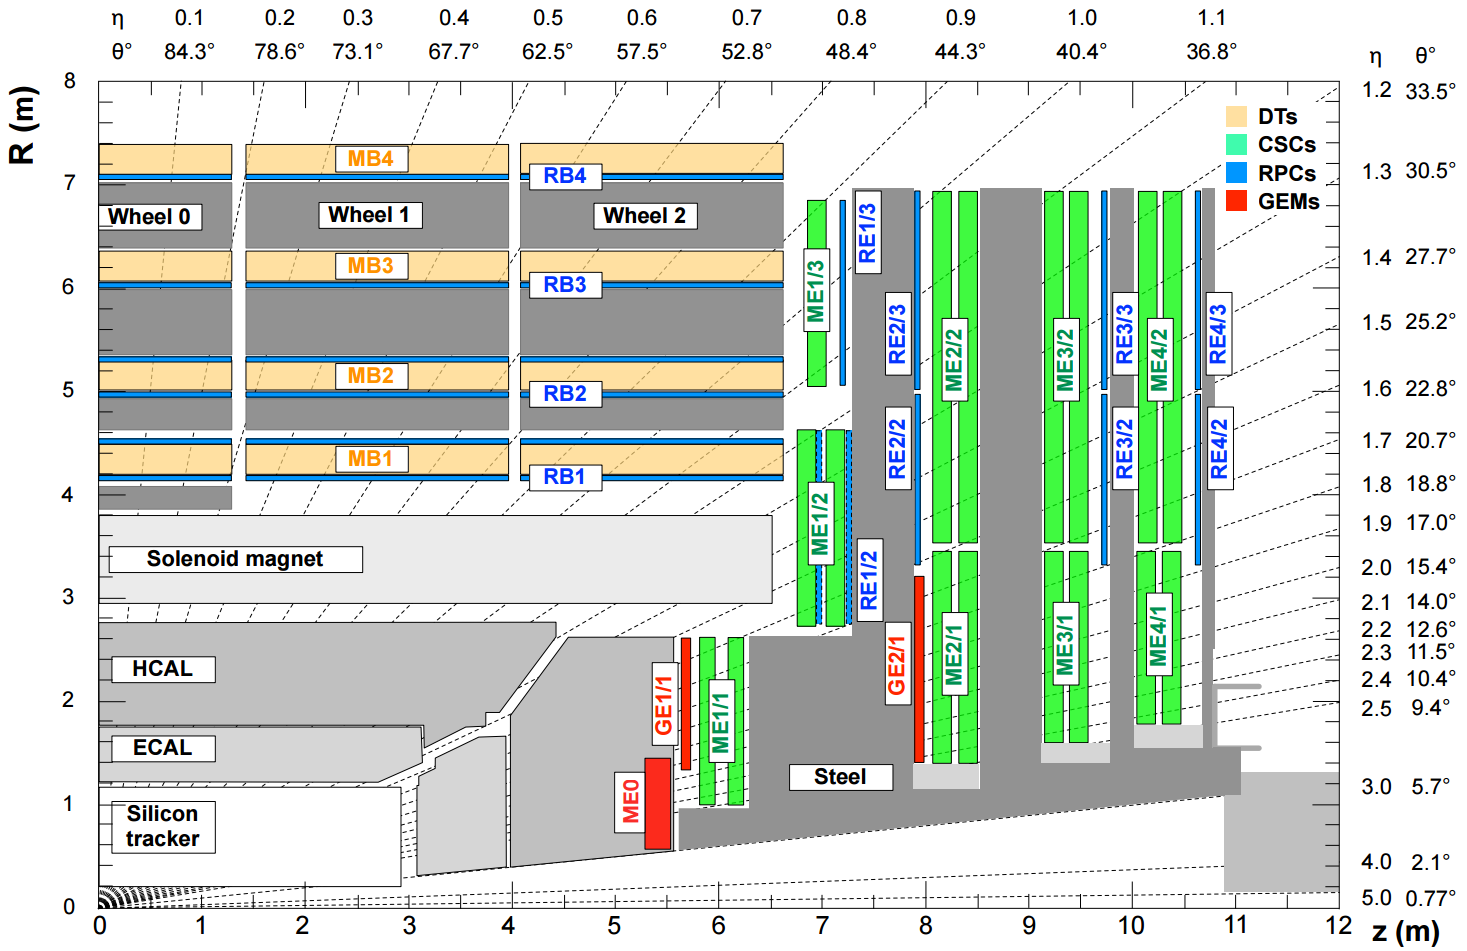
\includegraphics[width=\textwidth]{img/II-1-gem/ls3.png}
      \caption{Longitudinal view of a quadrant of CMS highlighting the location of the GE1/1, GE2/1, and ME0 detectors colored in red within the muon spectrometer. DTs are represented in yellow, CSCs in green, and RPCs in blue \cite{Thierry:2065693}.}
      \label{fig:II-1-ls3}
    \end{figure}
